\section{\label{sec:dirn}Directionality from Inverse Beta Decay}
% \section{\label{sec:dirn}Directionality from IBD}

%% definition
\subsection{\label{subsec:dirn_def}Definition}
 We start with defining the coordinate system used herein.  Under the assumption that the sources in question are located in the same horizontal plane as the detector (neither in the sky nor deep underground relative to the observation point), we focus on determination of the azimuthal direction. Note that some of the background from distant reactors will be substatially out of plane we get some small relief from reactors well below the horizon. Azimuth
 
% src-dtr
\begin{figure}[ht]
  \begin{center}
    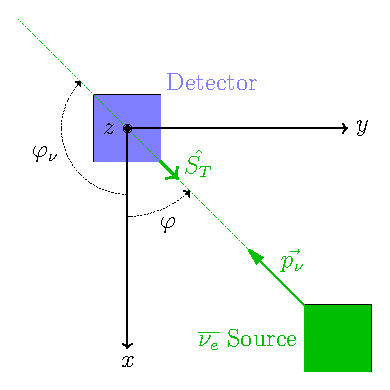
\includegraphics[width=0.6\linewidth]{figures/phi.eps}
    \caption{Illustration of Key Directional Quantities}
    \label{fig:phi_def}
  \end{center}
\end{figure}

\begin{gather}
    \varphi\ \equiv\ \varphi_{source}\ =\ \varphi_{\nu} \pm 180^o \label{eq:phi_def},\\
    \varphi_{\nu}\ =\ \arctan \left(\frac{p_{\perp}}{p_{\parallel}} \right)\ =\ \arctan \left( \frac{\Delta y}{\Delta x} \right) \label{eq:phi_calc} 
\end{gather}

In detector physics, \emph{directionality} refers to the ability of a detector to determine the incident direction of an incoming particle, and by extension to infer the direction pointing from the detector to the particle's source.
Fig.~\ref{fig:phi_def} illustrates this concept as applied to a detector attempting to reconstruct the direction \snu\ to the source of the incoming antineutrinos.
In the case shown here, the source is assumed to be located on the horizon relative to the detector (i.e., $z_{Detector}\ =\ z_{Source}$), so this problem reduces to reconstructing the azimuthal angle $\varphi$, which can be found as given in~\ref{eq:phi_def} and~\ref{eq:phi_calc}.


%% method
\subsection{\label{subsec:dirn_meth}Method}
\begin{figure}[ht]
\centering
  \begin{subfigure}{0.8\linewidth}
    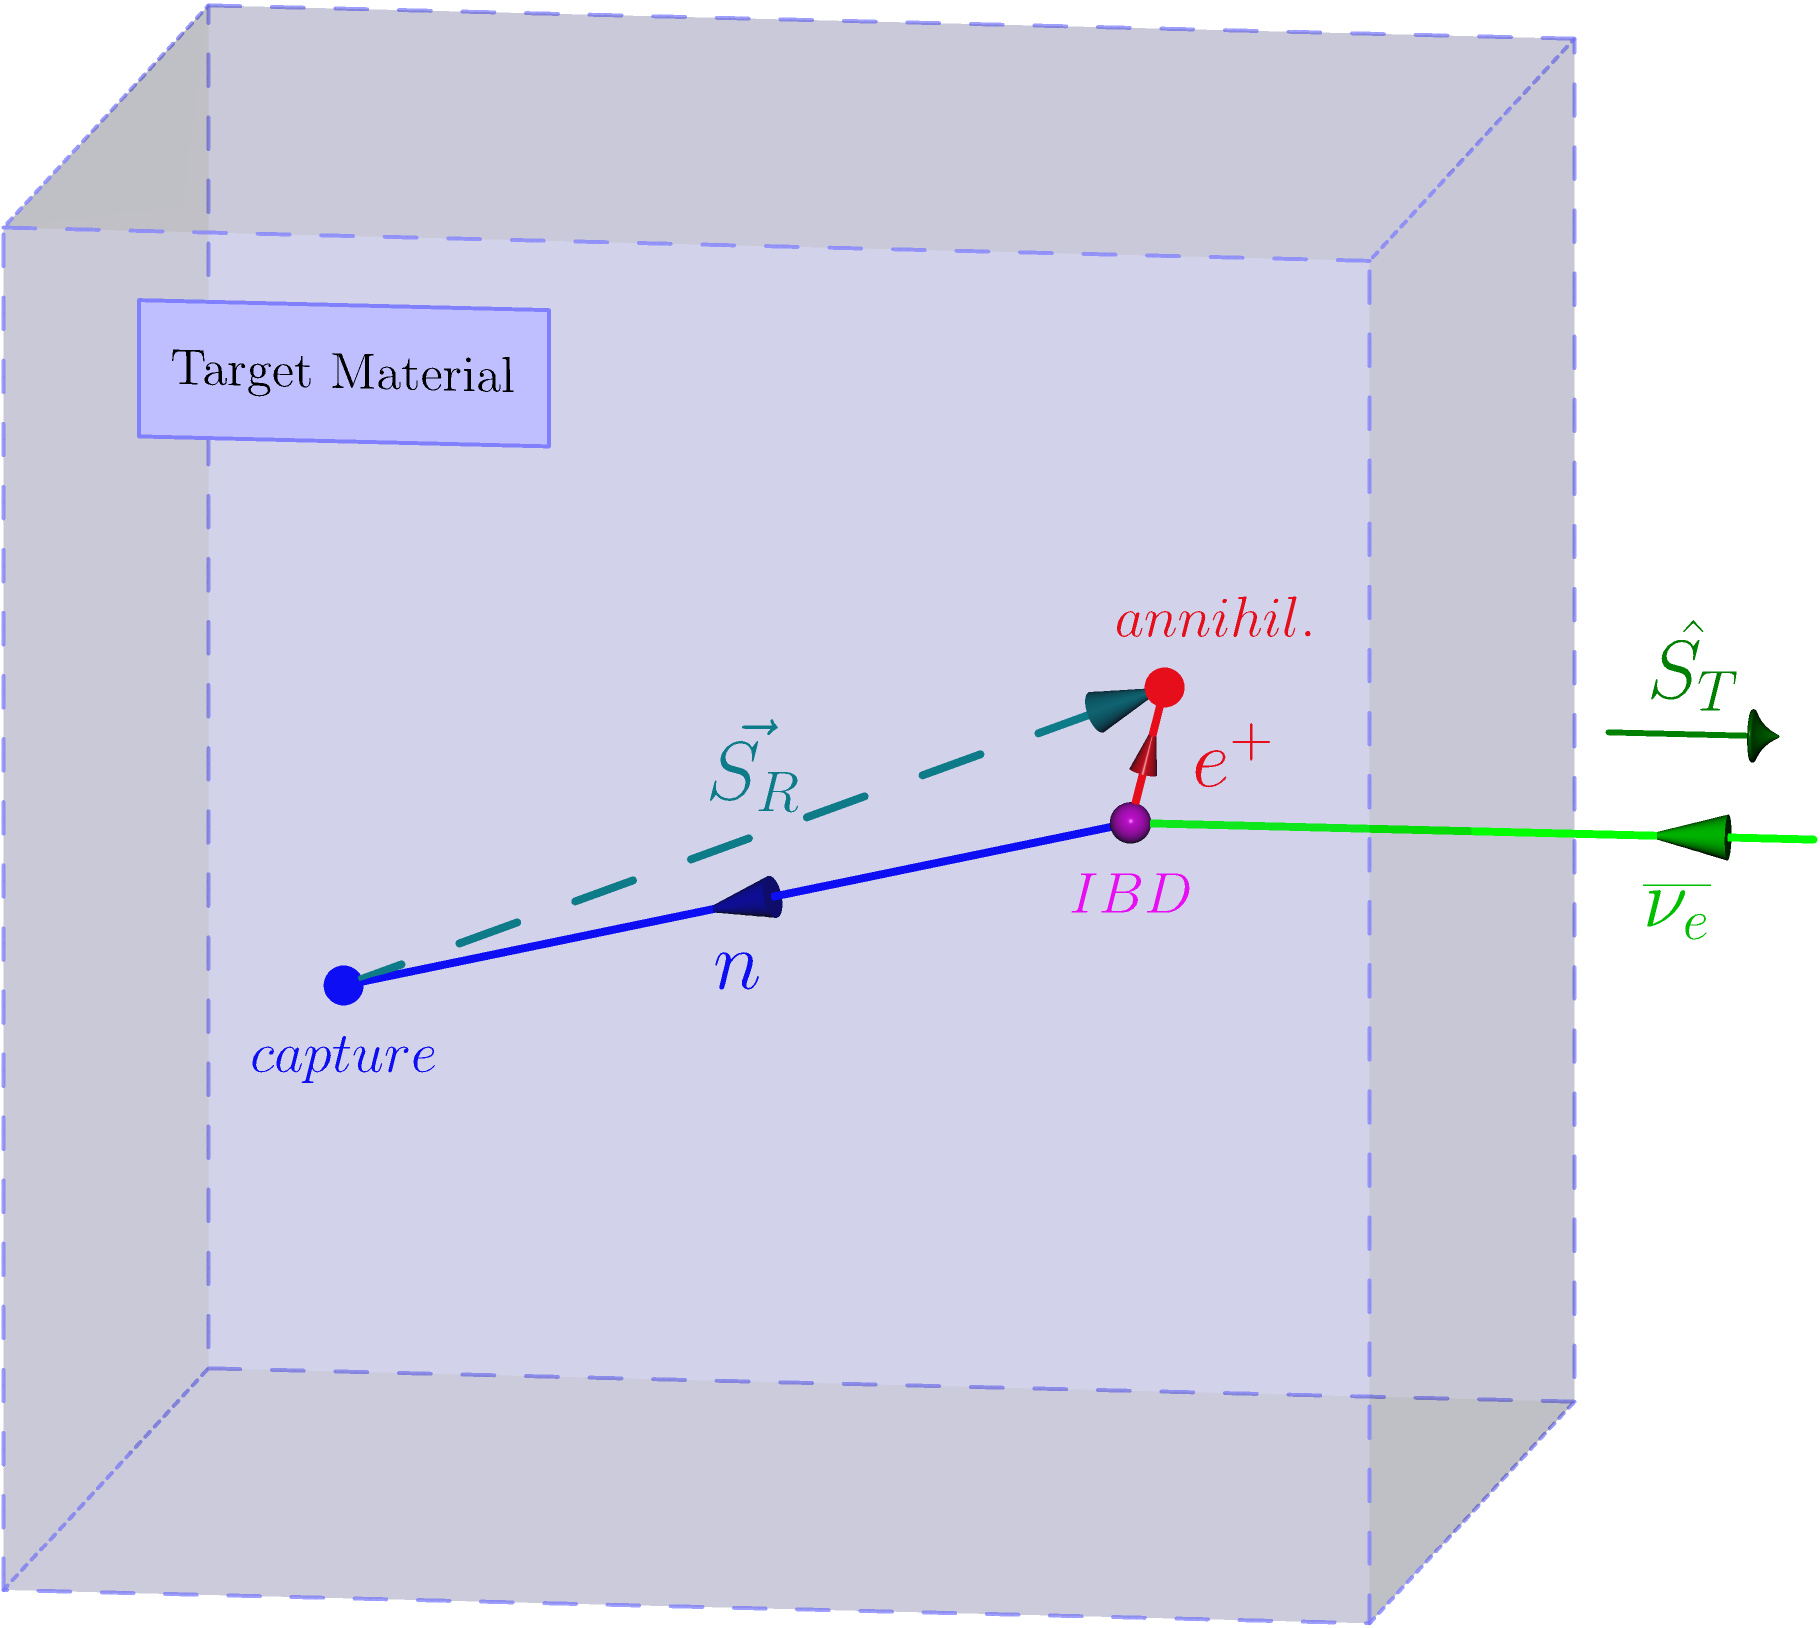
\includegraphics[width=\linewidth]{figures/recon.png}
    \caption{Definition of Reconstruction Vector $\vec{S_R}$}
    \label{fig:recon}
    % \vspace*{0.8cm}
  \end{subfigure}
  \begin{subfigure}{0.8\linewidth}
    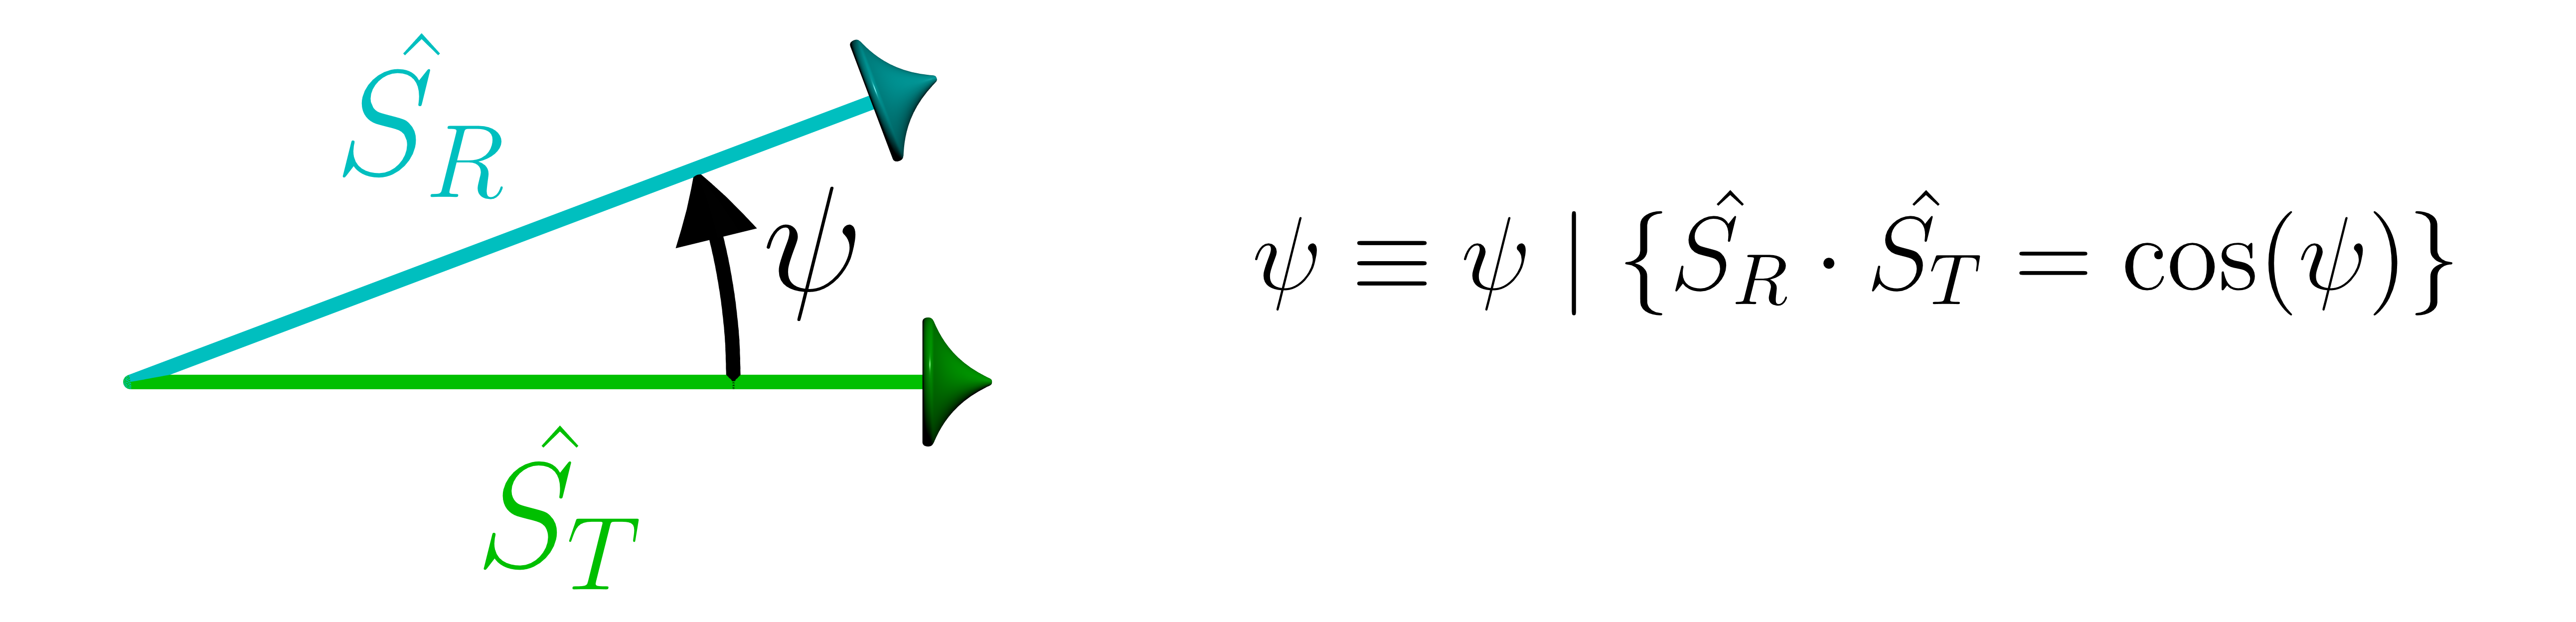
\includegraphics[width=\linewidth]{figures/psi.png}
    % \caption{Definition of $\psi$ as the Angle Between the True (\snu) and\\Reconstructed (\rhat) Source Directions}
    \caption{Definition of $\psi$ as the Angle Between the True (\snu) and Reconstructed (\rhat) Source Directions}
    \label{fig:psi}
  \end{subfigure}
  \caption{Method for IBD Directionality and Definition of Angle $\psi$} between prompt positron production and delayed neutron capture locations.
  \label{fig:dirn_def}
\end{figure}

The kinematics of \ibd\ have two primary consequences for our detection sceme:
\begin{enumerate}
  \item The \epc\ receives most of the \nbc's kinetic energy, though it is scattered widely (think of a ping-pong ball scattering off a bowling ball) and
  \item The \nnc\ receives most of the \nbc's momentum and therefore its directional information.
\end{enumerate}
\textbf{The key task for \ibd\ directionality is therefore to find the \nnc's displacement from its production at the \ibd\ vertex to its capture location.}
Because the \epc's displacement from production (also at the \ibd\ vertex) to annihilation is typically much shorter than the \nnc's capture displacement, we can reliably use the location of \epc\ annihilation to approximate the location of the \ibd\ vertex.
The method for extracting directional information from an \ibd\ detector is then to draw a vector from the location of neutron capture to the location of positron annihilation. % for each event. % that registers as an \ibd\ candidate.%, as shown in Fig.~\ref{fig:dirn_def}.
This vector, which we will notate as \rec, represents the reconstructed direction to the antineutrino source.
The true direction from the detector back to the neutrino source will be indicated by the unit vector \snu.
This process for a single typical \ibd\ event is shown in Fig.~\ref{fig:recon}:
\begin{enumerate}
  \item An incoming \nbc\ enters an arbitrary region of the detector's target material
  \item The \nbc\ undergoes \ibd\ by interacting with a $p^+$ in the target material, producing a \nnc\ and an \epc at the expense of the neutron-proton mass difference of 1.8 MeV in incoming neutrino energy.
  \item The \epc\ travels a short distance and annihilates with an $e^-$; this is called the \emph{prompt event} The positron leaves a trail of ionization for several {cm} prior to annihilation usually into two {511 keV} gammas.  The back-to-back gammas have ranges of many {cm} in the target materials and usually depart the region.  (They may or may not be recorded in the detector, but are identified as travelling at the speed of light, distinguishing the event from some backgrounds). We do not consider these in the present analysis.
  
  \item Meanwhile, the \nnc\ undergoes a series of intermediate scattering steps (omitted in the Figure for clarity) and eventually captures, either on a free proton ({np}) or usually on a nucleus of dopant material; this is called the delayed event and may be a few microseconds later, as compared to the prompt event (delayed by several {\it ns} from the neutrino interaction).
  \item We draw our vector \rec\ from \nnc-capture to \epc-annihilation
  \item Finally, we take as our reconstructed source direction $\rhatm \equiv \recm / \| \recm \|$
\end{enumerate}
The average of \rhat\ over a large number of events will then increasingly tend toward \snu.
The magnitude $\| \recm \|$ gives us the neutron's approximate capture distance.
We will sometimes be interested in this, but for directional purposes it is often convenient to simply use the corresponding unit vector, \rhat.
We can also define the quantity $\psi$ as the angle between \rhat\ and \snu, as shown in Fig.~\ref{fig:psi} and according to the following:

% definition of psi
\begin{equation}
  \psi\ \equiv\ \psi \mid \{ \rhatm \cdot \snum \} = \cos(\psi)
\end{equation}

% % explanation of cos[psi] -- TODO: maybe save this explanation for the Results?
% \begin{figure}[ht]
%   \begin{center}
%     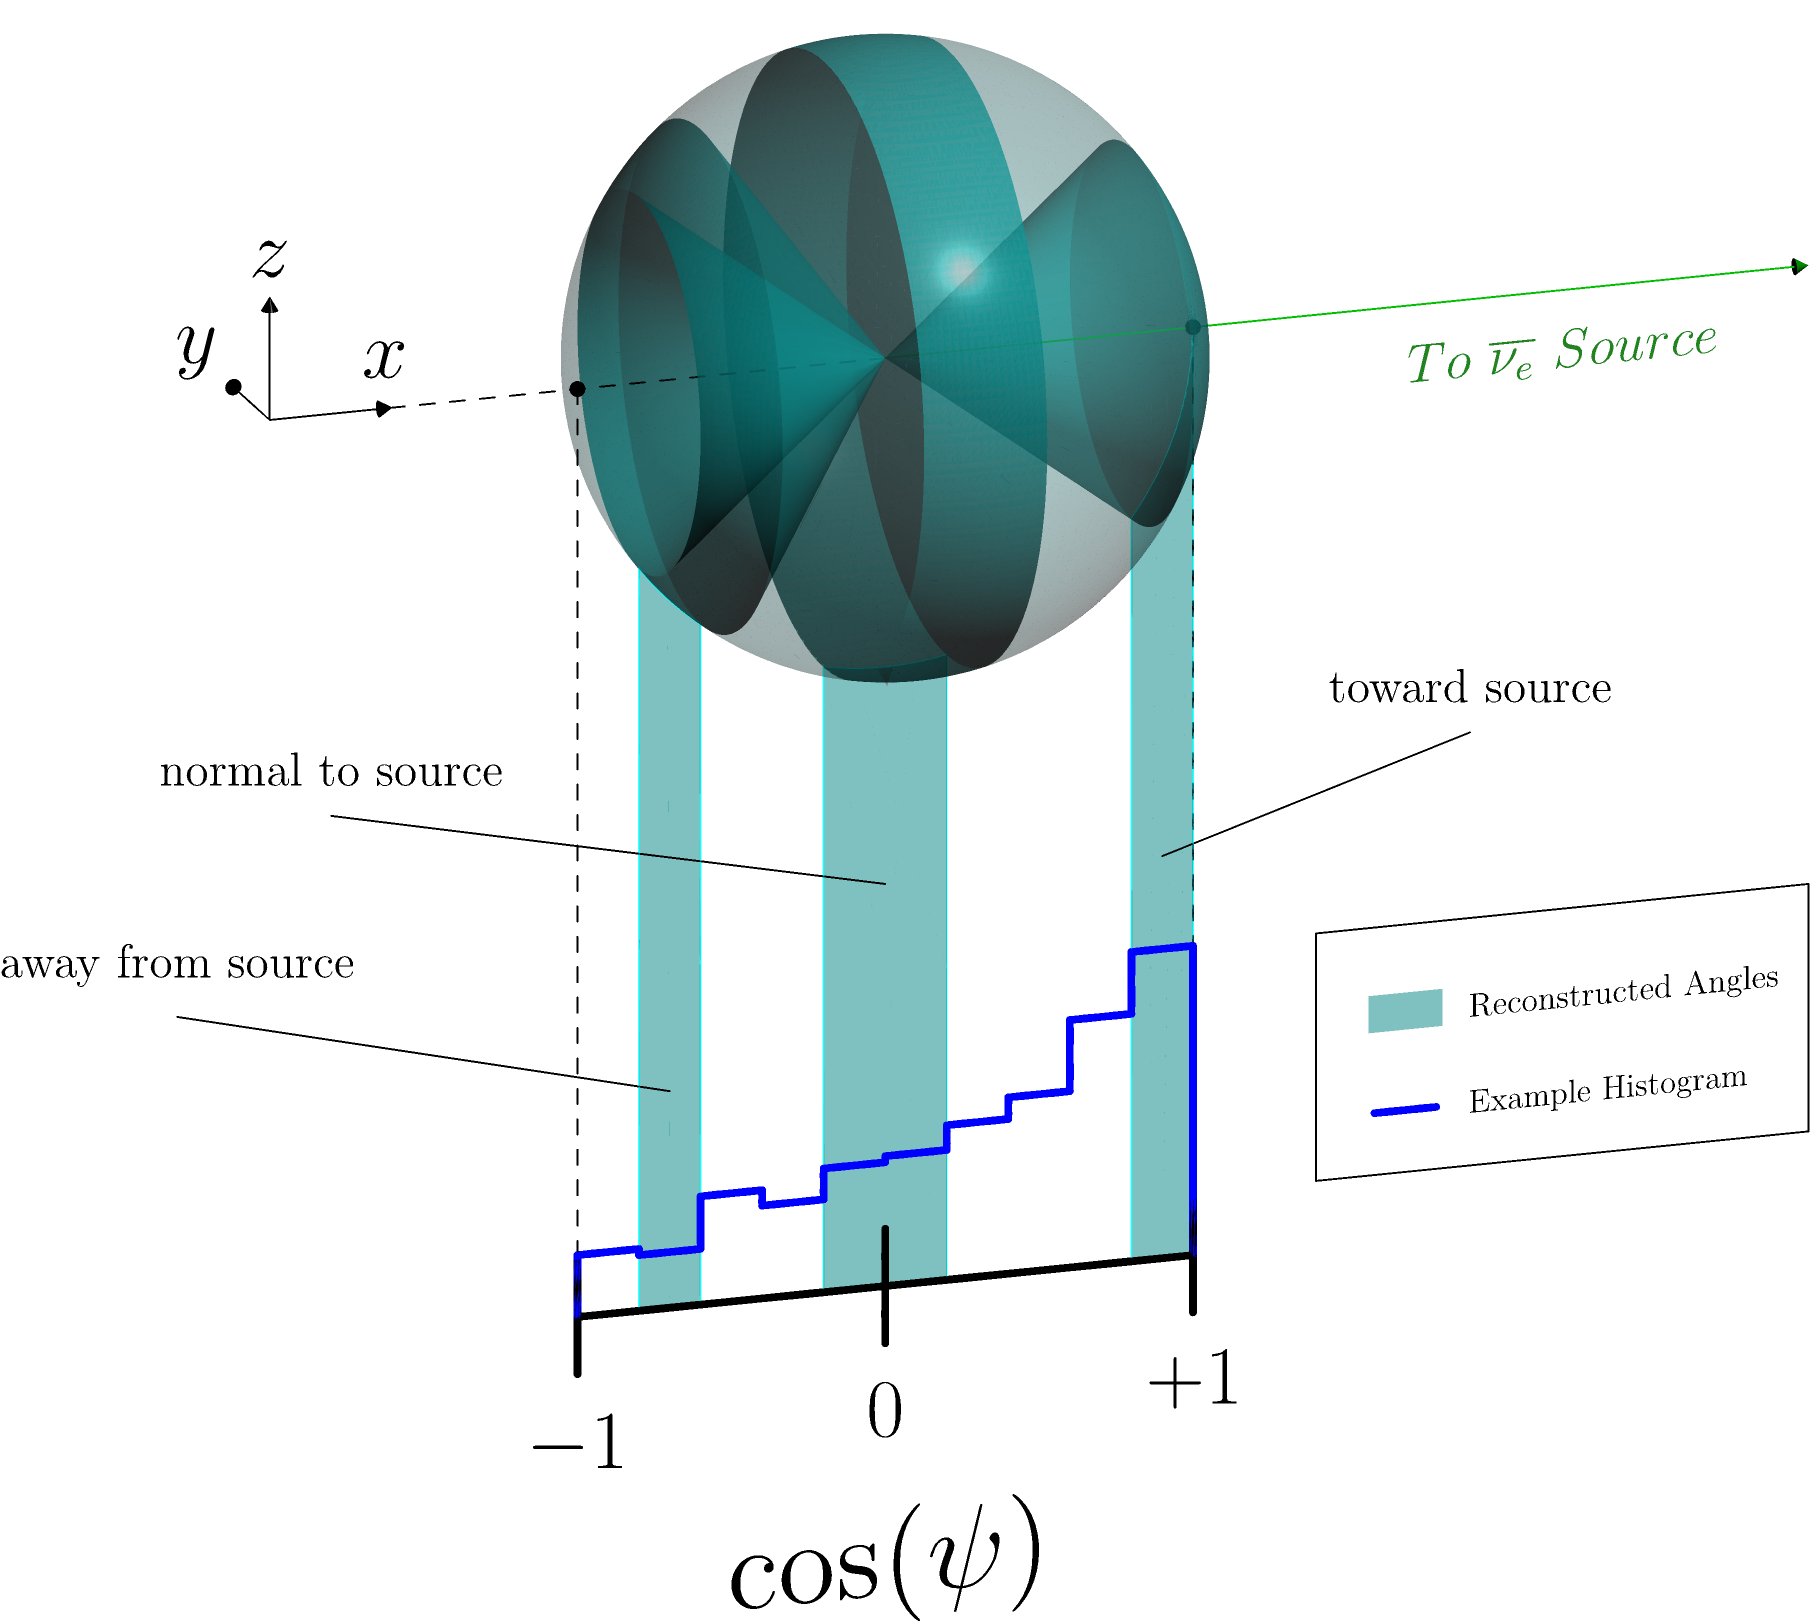
\includegraphics[width=0.9\linewidth]{figures/cospsi.png}
%     \caption{\textbf{Physical Meaning of Cos$\bm{(\psi)}$ Distributions}}
%     \label{fig:cospsi}
%   \end{center}
% \end{figure}
%
% The angle $\psi$ \dash or more specifically, its cosine \dash is especially helpful for evaluating a detector's directional performance.
% The quantity $\cos(\psi)$ for a given event or set of events gives a single value on the interval $\{-1,+1\}$ that reflects the degree of agreement between \rhat\ and \snu, as illustrated in Fig.~\ref{fig:cospsi}.
% Values near $-1$ indicate a reconstructed direction pointing away from the true source direction; values near $0$, perpendicular to the true source direction; and values near $+1$, toward the true source direction.
% For example, events in the leftmost shaded region in Fig.~\ref{fig:cospsi} (i.e., the second bin from the left in the example histogram) correspond to reconstructed angles falling within the solid angle between the two cones defined by $\cos(\psi) = -0.8$ and $\cos(\psi) = -0.6$, or $\psi \approx 143^o$ and $\psi \approx 127^o$.


%% stats
\subsection{\label{subsec:dirn_stats}Statistics}
The determination of the direction of the incoming \nbc\ is an inherently stochastic process.
This is because of the scattering undergone by the neutron during its moderation / thermalization phase. % which is discussed in \S\ref{subsec:n0_therm}.
This scattering is a \emph{nearly}-isotropic random-walk after the first scattering, with only a slight bias in the forward direction of neutrino travel.
The neutron's capture displacement (and consequently \rhat) for any particular event will then be in a nearly-random direction, and it is therefore only the average of \rhat\ over a substantial number of events that will reliably point in a direction near \snu\ and give a meaningful result for the direction to the neutrino source.
This is true even for cases in which the \nnc-scattering region can be separated from the \epc-annihilation region, as will be discussed in detail in \S\ref{subsec:sep}.
The results in~\cite{Vogel:1999zy} also indicate that on average, the \epc\ will have a slight bias to leave the \ibd\ interaction
  heading in the backward direction relative to the incoming \nbc.
%TODO: Mention that this could be useful, but no one's done it yet.


%% other instruments
\subsection{\label{subsec:dirn_prev}Other Relevant current, past and near future Detectors}

%The first measurement of incoming \nb\ direction using this (or any) approach was determined and published
%  by the collaboration on the Double CHOOZ experiment~\cite{PhysRevD.61.012001}.
\textbf{Previous} \quad
The first experiment to successfully demonstrate directional detection of electron antineutrinos via \ibd\ was the Chooz experiment, which used $\sim 2700$ \ibd\ events to ``[locate] an antineutrino source to within a cone of half-aperture $\approx 22^o$ at the 68\% C.L.'' (confidence level)~\cite{Apollonio:1999jg}.
The \dc\ experiment then improved on this result, acquiring $\sim$ 8200 \ibd\ events and reducing the cone to half-aperture $\approx 6^o$~\cite{Caden:2012aap}. % Caden presentation <---> which paper??

\textbf{Concurrent, Under construction and future} \quad
Other collaborations working along these lines include the PROSPECT~\cite{Ashenfelter:2013oaa}\cite{Ashenfelter:2015tpm} and Chinese Daya Bay~\cite{DayaBay:2012aa} experiments(both presently not operating) Korean RENO, Double Chooz, and Borexino Experiments have concluded. KamLAND and SuperKamiokande are operating.but neither have the resolution to resolve IBD directions. The HyperK experiment in Japan is under construction but appears to not being able to do IBD directionalit.  THe JUNO project in China is under construction and hopefully will soon operate (in 2023). (We need to say something about its directional capabilities... some work to do here.)

